%%%%%%%%%%%%%%%%%%%%%%%%%%%%%%%%%% Preâmbulo %%%%%%%%%%%%%%%%%%%%%%%%%%%%%%%%%% 

\documentclass[12pt,a4paper]{article}\usepackage[]{graphicx}\usepackage[]{color}
% maxwidth is the original width if it is less than linewidth
% otherwise use linewidth (to make sure the graphics do not exceed the margin)
\makeatletter
\def\maxwidth{ %
  \ifdim\Gin@nat@width>\linewidth
    \linewidth
  \else
    \Gin@nat@width
  \fi
}
\makeatother

\definecolor{fgcolor}{rgb}{0.345, 0.345, 0.345}
\newcommand{\hlnum}[1]{\textcolor[rgb]{0.686,0.059,0.569}{#1}}%
\newcommand{\hlstr}[1]{\textcolor[rgb]{0.192,0.494,0.8}{#1}}%
\newcommand{\hlcom}[1]{\textcolor[rgb]{0.678,0.584,0.686}{\textit{#1}}}%
\newcommand{\hlopt}[1]{\textcolor[rgb]{0,0,0}{#1}}%
\newcommand{\hlstd}[1]{\textcolor[rgb]{0.345,0.345,0.345}{#1}}%
\newcommand{\hlkwa}[1]{\textcolor[rgb]{0.161,0.373,0.58}{\textbf{#1}}}%
\newcommand{\hlkwb}[1]{\textcolor[rgb]{0.69,0.353,0.396}{#1}}%
\newcommand{\hlkwc}[1]{\textcolor[rgb]{0.333,0.667,0.333}{#1}}%
\newcommand{\hlkwd}[1]{\textcolor[rgb]{0.737,0.353,0.396}{\textbf{#1}}}%
\let\hlipl\hlkwb

\usepackage{framed}
\makeatletter
\newenvironment{kframe}{%
 \def\at@end@of@kframe{}%
 \ifinner\ifhmode%
  \def\at@end@of@kframe{\end{minipage}}%
  \begin{minipage}{\columnwidth}%
 \fi\fi%
 \def\FrameCommand##1{\hskip\@totalleftmargin \hskip-\fboxsep
 \colorbox{shadecolor}{##1}\hskip-\fboxsep
     % There is no \\@totalrightmargin, so:
     \hskip-\linewidth \hskip-\@totalleftmargin \hskip\columnwidth}%
 \MakeFramed {\advance\hsize-\width
   \@totalleftmargin\z@ \linewidth\hsize
   \@setminipage}}%
 {\par\unskip\endMakeFramed%
 \at@end@of@kframe}
\makeatother

\definecolor{shadecolor}{rgb}{.97, .97, .97}
\definecolor{messagecolor}{rgb}{0, 0, 0}
\definecolor{warningcolor}{rgb}{1, 0, 1}
\definecolor{errorcolor}{rgb}{1, 0, 0}
\newenvironment{knitrout}{}{} % an empty environment to be redefined in TeX

\usepackage{alltt}
\usepackage[utf8]{inputenc}
\usepackage{amsmath}
\usepackage{amsfonts}
\usepackage{amssymb}
\usepackage{makeidx}
\usepackage{graphicx}
\usepackage{booktabs}
\usepackage{xcolor}
\usepackage{bm}
\usepackage{float}
\usepackage[margin=1.5in]{geometry}
\usepackage[normalem]{ulem}
\useunder{\uline}{\ul}{}
\let\lctau\tau % save the lowercase of '\tau'
\renewcommand{\tau}{\scalerel*{\lctau}{X}}
\renewcommand{\tablename}{\textbf{Tabela}}

\usepackage{hyperref}
\hypersetup{
    colorlinks,
    citecolor=black,
    filecolor=black,
    linkcolor=black,
    urlcolor=black
}

\renewcommand{\contentsname}{Sumário} 

\title{MLG - Trabalho 2}
\author{José Carlos Soares Junior }
\date{Matrícula: 2017100732}
\IfFileExists{upquote.sty}{\usepackage{upquote}}{}
\begin{document}
\begin{titlepage}
	\begin{center}
	
	%\begin{figure}[!ht]
	%\centering
	%\includegraphics[width=2cm]{c:/ufba.jpg}
	%\end{figure}

		\Huge{UNIVERSIDADE FEDERAL DO ESPÍRITO SANTO}\\
		\large{CENTRO DE CIÊNCIAS EXATAS}\\ 
		\large{DEPARTAMENTO DE ESTATÍSTICA}\\ 
\vspace{15pt}
        
        \vspace{85pt}
        
		\textbf{\LARGE{Modelagem dos dados de 2013 referentes às notificações de dengue no estado do Espírito Santo}}
		\title{\large{Título}}
	%	\large{Modelo\\
     %   		Validação do modelo clássico}
			
	\end{center}
\vspace{1,5cm}
	
	\begin{flushright}

   \begin{list}{}{
      \setlength{\leftmargin}{4.5cm}
      \setlength{\rightmargin}{0cm}
      \setlength{\labelwidth}{0pt}
      \setlength{\labelsep}{\leftmargin}}

      \item Segundo trabalho da disciplina de MLG ministrado pelo Prof. Dr. Saulo Morellato.

      \begin{list}{}{
      \setlength{\leftmargin}{0cm}
      \setlength{\rightmargin}{0cm}
      \setlength{\labelwidth}{0pt}
      \setlength{\labelsep}{\leftmargin}}

			\item Alunos: \
            \item Orientador: Prof. Dr. Saulo Morellato\

      \end{list}
   \end{list}
\end{flushright}
\vspace{1cm}
\begin{center}
		\vspace{\fill}
		 Abril\\
		 2021
			\end{center}
\end{titlepage}
\newpage

%%%%%%%%%%%%%%%%%%%%%%%%%%%%%%%%%% Pacotes %%%%%%%%%%%%%%%%%%%%%%%%%%%%%%%%%% 



\tableofcontents  % sumário

% Formato do chunk a ser usado:



%%%%%%%%%%%%%%%%%%%%%%%%%%% Descrição dos dados %%%%%%%%%%%%%%%%%%%%%%%%%%%%%% 

\newpage
\section{\textbf{{\LARGE\textbf{Descrição dos dados}}}}

\textbf{IntCdAtBca} - Proporção de internações por condições sensíveis à Atenção Basica;

\noindent
\textbf{CobCondSaud} - Cobertura de acompanhamento das condicionalidades de saúde do Programa Bolsa Família;

\noindent
\textbf{CobAtBas} - Cobertura das equipes atenção básica municipal expresso em percentual da cobertura populacional alcançada pela Atenção Básica;

\noindent
\textbf{temp} - temperatura média anual;

\noindent
$\mathbf{temp\_p10}$ - percentil $10$ das temperaturas durante o ano;

\noindent
$\mathbf{temp\_p90}$ - percentil $90$ das temperaturas durante o ano;

\noindent
\textbf{precip} - precipitação pluviométrica acumulada anual;

\noindent
\textbf{umid} - média anual da umidade relativa do ar;

\noindent
$\mathbf{umid\_p10}$ - percentil $10$ da umidade relativa do ar durante o ano;

\noindent
$\mathbf{umid\_p90}$ - percentil $90$ da umidade relativa do ar durante o ano;

\noindent
\textbf{alt} - altitude da sede municipal;

\noindent
\textbf{ifdm\_saude} - Índice Firjan de Desenvolvimento Municipal-IFDM para saúde;

\noindent
\textbf{ifdm\_edu} - Índice Firjan de Desenvolvimento Municipal-IFDM para educação;

\noindent
\textbf{ifdm\_emprend} - Índice Firjan de Desenvolvimento Municipal-IFDM de emprego e renda;

\noindent
\textbf{cobveg} - índice de cobertura vegetal;

\noindent
\textbf{expcosteira} - ídice de exposição costeira;

\noindent
\textbf{ivc} - índice de vulnerabilidade climática;

\noindent
\textbf{pobr} - proporção de pobres;

\noindent
\textbf{ExpAnosEstud} - expectativa de anos de estudo;

\noindent
\textbf{urb} - proporção da população que reside em zona urbana;

\noindent
$\mathbf{menor15}$ - proporção da população com menos de $15$ anos;

\noindent
$\mathbf{maior65}$ - proporção da população com mais de $65$ anos;

\noindent
\textbf{adultos} - proporção da população entre $15$ e $65$ anos;

\noindent
\textbf{pop} - população do município;

\noindent
\textbf{area} - área do município;

\noindent
\textbf{dens} - densidade populacional (pop\/area);

\noindent
\textbf{id} - identificação;

\noindent
\textbf{ano} - ano referente às informações; e

\noindent
\textbf{dengue} - número de notificações municipais de dengue.

%%%%%%%%%%%%%%%%%%%%%%%%%%%%%%%%%% Descritiva %%%%%%%%%%%%%%%%%%%%%%%%%%%%%%%%%% 

\newpage
\section{{\LARGE\textbf{Análise exploratória}}}

%%%%%% Notificações de dengue por municipio %%%%%%%

\begin{knitrout}
\definecolor{shadecolor}{rgb}{0.969, 0.969, 0.969}\color{fgcolor}

{\centering 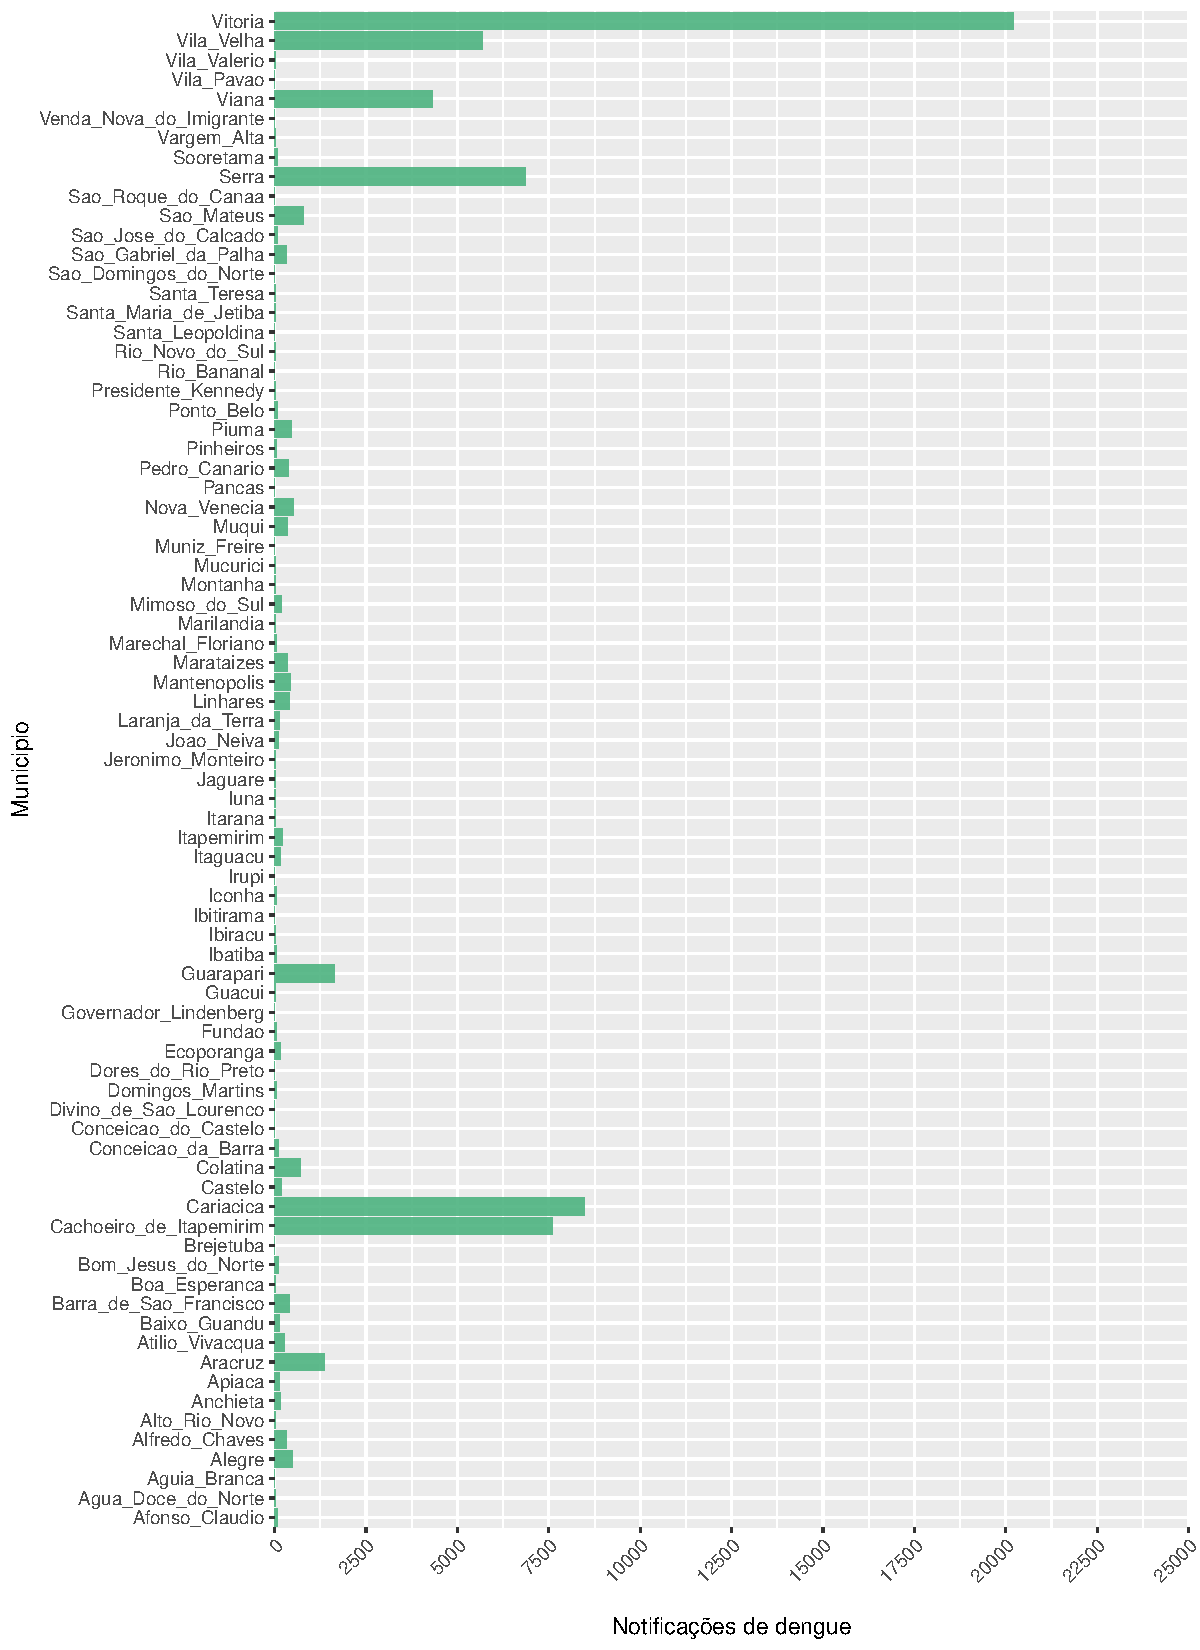
\includegraphics[width=\maxwidth]{figure/unnamed-chunk-3-1} 

}



\end{knitrout}
\textbf{Figura 1:} Notificações de dengue por municípios do estado do Espírito Santo.

%%%%%%% Grafico de correlação %%%%%%%

\begin{knitrout}
\definecolor{shadecolor}{rgb}{0.969, 0.969, 0.969}\color{fgcolor}
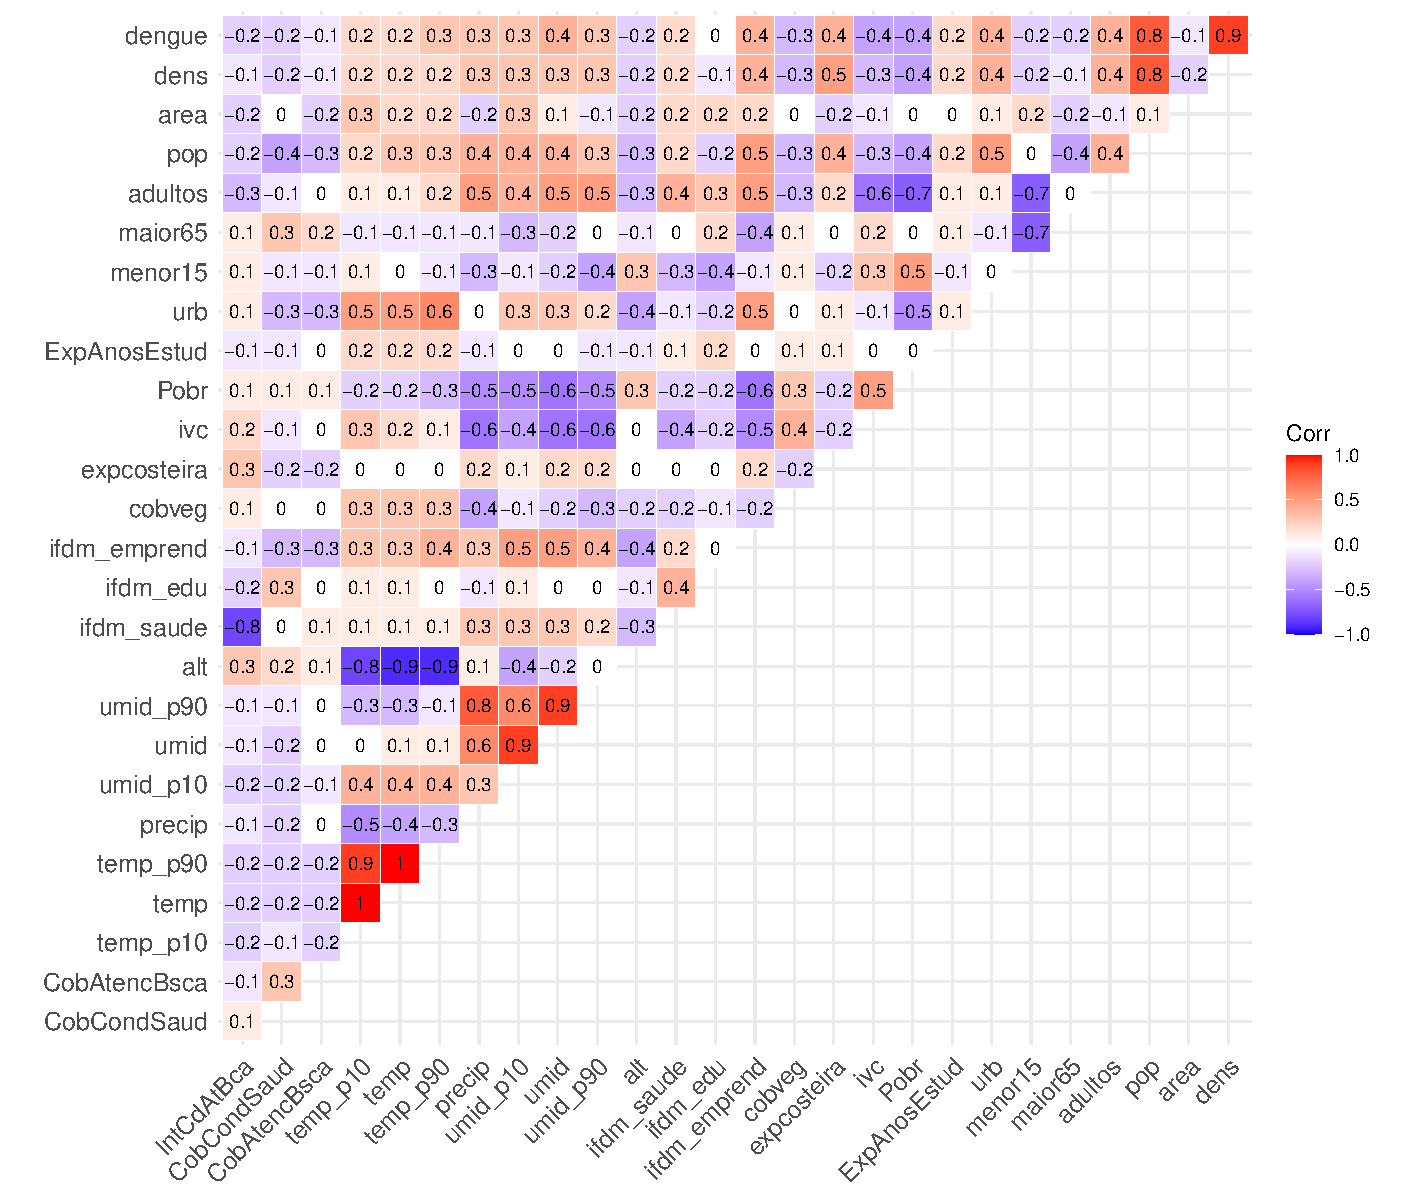
\includegraphics[width=\maxwidth]{figure/unnamed-chunk-4-1} 

\end{knitrout}
\textbf{Figura 2:} Gráfico de correlação entre as covariáveis.

\newpage
\section{{\LARGE\textbf{Construção do modelo}}}

A primeira coisa a se fazer para termos um modelo de regressão é verificar se é possível utilizar a regressão linear, sendo que, nesse modelo a nossa variável resposta tem de apresentar uma distribuição aproximadamente normal.

Como temos a nossa variável de interesse como um dado de contagem, sendo esses dados com valores baixos, não é correto que ajustemos um modelo linear simples, sendo então necessário um modelo específico, no caso temos duas distribuições principais que podem ser melhores ajustes:

\begin{itemize}
  \item Poisson
  \item Binomial Negativa
\end{itemize}

\subsection{\textbf{Modelo Poisson}}

Como vimos, a variável independente do modelo possui um formato que condiz com o de uma distribuição Poisson, temos, também que $Y_i$ são independentes $\forall i \leq n$, onde cada unidade experimental é o município.

\subsubsection{\textbf{Definição do modelo}}

Utilizando uma função de ligação logarítmica temos um modelo inicial utilizando todas as variáveis na forma sistemática abaixo

$$log(\lambda_i)=\alpha+\beta_1{x_1}_i+\beta_2{x_2}_i+\cdots+\beta_{26}{x_{26}}_i$$

\subsubsection{\textbf{Modelo considerando todas as covariáveis}}

Ajustando um modelo com todas as $26$ covariáveis e realizando a seleção de variáveis pelo método \_\_AIC\_\_ temos suas informações abaixo:

\begin{knitrout}
\definecolor{shadecolor}{rgb}{0.969, 0.969, 0.969}\color{fgcolor}\begin{kframe}
\begin{verbatim}

Call:
glm(formula = dengue ~ IntCdAtBca + CobCondSaud + CobAtencBsca + 
    temp_p10 + temp + temp_p90 + precip + umid_p10 + umid + umid_p90 + 
    alt + ifdm_saude + ifdm_edu + ifdm_emprend + cobveg + expcosteira + 
    ivc + Pobr + ExpAnosEstud + urb + menor15 + maior65 + pop + 
    area + dens, family = poisson, data = data)

Deviance Residuals: 
    Min       1Q   Median       3Q      Max  
-76.799   -8.593   -3.737    2.188   80.479  

Coefficients:
               Estimate Std. Error z value Pr(>|z|)    
(Intercept)   5.625e+00  5.033e-01  11.177  < 2e-16 ***
IntCdAtBca   -1.841e-02  7.551e-04 -24.376  < 2e-16 ***
CobCondSaud  -1.122e-02  2.981e-04 -37.640  < 2e-16 ***
CobAtencBsca -8.239e-04  2.413e-04  -3.415 0.000637 ***
temp_p10      1.541e+00  2.921e-02  52.764  < 2e-16 ***
temp         -1.732e+00  4.962e-02 -34.911  < 2e-16 ***
temp_p90      4.375e-01  2.323e-02  18.835  < 2e-16 ***
precip        1.020e-03  2.390e-05  42.688  < 2e-16 ***
umid_p10     -3.788e-02  7.191e-03  -5.267 1.39e-07 ***
umid         -2.660e-01  1.490e-02 -17.858  < 2e-16 ***
umid_p90      3.570e-01  9.558e-03  37.357  < 2e-16 ***
alt          -1.478e-03  6.399e-05 -23.103  < 2e-16 ***
ifdm_saude   -4.640e-02  1.012e-03 -45.845  < 2e-16 ***
ifdm_edu      1.186e-02  1.532e-03   7.738 1.01e-14 ***
ifdm_emprend -1.883e-02  4.796e-04 -39.255  < 2e-16 ***
cobveg       -4.985e-03  2.213e-04 -22.522  < 2e-16 ***
expcosteira  -1.826e-02  2.070e-04 -88.190  < 2e-16 ***
ivc          -2.312e-02  3.151e-04 -73.368  < 2e-16 ***
Pobr          1.084e-01  2.277e-03  47.591  < 2e-16 ***
ExpAnosEstud  1.625e-01  1.060e-02  15.325  < 2e-16 ***
urb           4.995e-02  5.676e-04  87.989  < 2e-16 ***
menor15      -3.528e-01  5.361e-03 -65.821  < 2e-16 ***
maior65      -3.859e-01  6.691e-03 -57.672  < 2e-16 ***
pop           4.913e-06  5.292e-08  92.841  < 2e-16 ***
area          2.482e-04  7.988e-06  31.069  < 2e-16 ***
dens          2.018e-04  7.718e-06  26.147  < 2e-16 ***
---
Signif. codes:  0 '***' 0.001 '**' 0.01 '*' 0.05 '.' 0.1 ' ' 1

(Dispersion parameter for poisson family taken to be 1)

    Null deviance: 630804  on 389  degrees of freedom
Residual deviance:  76437  on 364  degrees of freedom
AIC: 78440

Number of Fisher Scoring iterations: 6
\end{verbatim}
\end{kframe}
\end{knitrout}

% FAZER TABELA NO LUGAR DO CHUNK ACIMA DE SER TEMPO.

Vemos que o desvio do resíduo é muito maior que seus graus de liberdade, o que indica um ajuste ruim. Para melhorar nosso modelo vamos reduzir sua dimensão, onde, pela análise descritiva, observamos que algumas covariáveis possuem baixa correlação com a variável resposta \_dengue\_, por esse motivo, as retiramos do modelo, são essas variáveis \_ifdm\_edu\_ e \_area\_.

Para impedir multicolinearidade observamos altas correlações entre pares de covariáveis, sendo as mais altas descritas a seguir:

\begin{table}[H]
\caption{Pares de covariáveis com as correlações mais altas identificadas:} 
\begin{center}
\begin{tabular}{c|c|c}
\hline
Variável 1                         & Variável 2      & Correlação                      \\ \hline
IntCdAtBca                         & $\mathbf{ifdm\_saude}$ & \multicolumn{1}{l}{-0.77960350} \\
temp\_p10                          & \textbf{alt}         & -0.821314067                    \\
temp\_p10                          & \textbf{temp}        & 0.993364738                     \\
temp\_p10                          & $\mathbf{temp\_p90}$   & 0.946850236                     \\
temp                               & $\mathbf{temp\_p90}$   & 0.976276719                     \\
\textbf{temp}                           & \textbf{alt}         & -0.852298080                    \\
$\mathbf{temp\_p90}$                      & alt             & -0.884910605                    \\
\textbf{precip}                         & umid\_p90       & 0.79257030                      \\
umid\_p10                          & \textbf{umid}        & 0.86471582                      \\
\textbf{umid}                           & umid\_p90       & 0.890202356                     \\
umid\_p90                          & \textbf{ivc}         & -0.63608509                     \\
$\mathbf{ifdm\_emprend}$                  & Pobr            & -0.62697421                     \\
Pobr                               & \textbf{adultos}     & -0.708001527                    \\
menor15                            & \textbf{maior65}     & -0.690958203                    \\
menor15                            & \textbf{adultos}     & -0.715345068                    \\
pop                                & \textbf{dens}        & 0.78260681                      \\ \hline
\end{tabular}
\end{center}
\end{table}

Para nosso modelo escolhemos, então, seguir com a variávei mais correlata com a variável resposta entre os pares da tabela acima, o que nos deixou com um modelo com as 15 variáveis abaixo:

\begin{itemize}
  \item CobCondSaud
  \item CobAtencBsca
  \item temp\_p$90$
  \item precip
  \item umid
  \item ifdm\_saude
  \item ifdm\_emprend
  \item cobveg
  \item expcosteira
  \item ivc
  \item ExpAnosEstud
  \item urb
  \item maior$65$
  \item adultos
  \item dens
\end{itemize}


\subsubsection{\textbf{Modelo com seleção de covariáveis}}

Com o modelo descrito acima obtivemos, também com a seleção de variáveis pelo \_AIC\_, os seguintes resultados:

\begin{knitrout}
\definecolor{shadecolor}{rgb}{0.969, 0.969, 0.969}\color{fgcolor}\begin{kframe}
\begin{verbatim}

Call:
glm(formula = dengue ~ CobCondSaud + CobAtencBsca + temp_p90 + 
    precip + umid + ifdm_saude + ifdm_emprend + cobveg + expcosteira + 
    ivc + ExpAnosEstud + urb + maior65 + adultos + dens, family = poisson, 
    data = data)

Deviance Residuals: 
    Min       1Q   Median       3Q      Max  
-79.650   -9.002   -3.851    2.948   89.358  

Coefficients:
               Estimate Std. Error  z value Pr(>|z|)    
(Intercept)  -1.780e+01  3.944e-01  -45.134   <2e-16 ***
CobCondSaud  -2.518e-02  2.579e-04  -97.636   <2e-16 ***
CobAtencBsca -1.032e-02  1.740e-04  -59.317   <2e-16 ***
temp_p90      4.684e-01  5.163e-03   90.728   <2e-16 ***
precip        1.003e-03  1.466e-05   68.392   <2e-16 ***
umid          2.474e-02  2.743e-03    9.022   <2e-16 ***
ifdm_saude   -2.334e-02  7.268e-04  -32.113   <2e-16 ***
ifdm_emprend -1.566e-02  4.009e-04  -39.069   <2e-16 ***
cobveg       -4.818e-03  1.943e-04  -24.799   <2e-16 ***
expcosteira  -2.103e-02  1.750e-04 -120.217   <2e-16 ***
ivc          -2.860e-02  2.502e-04 -114.313   <2e-16 ***
ExpAnosEstud  2.863e-01  8.079e-03   35.436   <2e-16 ***
urb           3.204e-02  4.126e-04   77.669   <2e-16 ***
maior65      -1.330e-01  3.252e-03  -40.898   <2e-16 ***
adultos       1.517e-01  3.737e-03   40.599   <2e-16 ***
dens          5.926e-04  6.096e-06   97.212   <2e-16 ***
---
Signif. codes:  0 '***' 0.001 '**' 0.01 '*' 0.05 '.' 0.1 ' ' 1

(Dispersion parameter for poisson family taken to be 1)

    Null deviance: 630804  on 389  degrees of freedom
Residual deviance: 101739  on 374  degrees of freedom
AIC: 103722

Number of Fisher Scoring iterations: 6
\end{verbatim}
\end{kframe}
\end{knitrout}

% FAZER TABELA NO LUGAR DO CHUNK ACIMA DE SER TEMPO.

Note que em comparação com o modelo completo, em teoria, pioramos a qualidade do ajuste, porém, tiramos as multicolinearidades, que podem ser observadas na tabela com os VIFs de cada variável por modelo abaixo:

\begin{knitrout}
\definecolor{shadecolor}{rgb}{0.969, 0.969, 0.969}\color{fgcolor}\begin{table}[H]

\caption{\label{tab:unnamed-chunk-7}Modelo com variáveis correlatas}
\centering
\begin{tabular}[t]{l|r}
\hline
  & VIF\\
\hline
IntCdAtBca & 3.340568\\
\hline
CobCondSaud & 4.516761\\
\hline
CobAtencBsca & 4.193826\\
\hline
temp\_p10 & 113.647345\\
\hline
temp & 301.402079\\
\hline
temp\_p90 & 59.161914\\
\hline
precip & 17.075523\\
\hline
umid\_p10 & 90.809074\\
\hline
umid & 227.462163\\
\hline
umid\_p90 & 52.120415\\
\hline
alt & 3.903644\\
\hline
ifdm\_saude & 6.531280\\
\hline
ifdm\_edu & 9.642008\\
\hline
ifdm\_emprend & 4.907702\\
\hline
cobveg & 7.685869\\
\hline
expcosteira & 9.610107\\
\hline
ivc & 8.212447\\
\hline
Pobr & 15.043009\\
\hline
ExpAnosEstud & 3.831969\\
\hline
urb & 7.619431\\
\hline
menor15 & 27.804045\\
\hline
maior65 & 17.626240\\
\hline
pop & 11.892503\\
\hline
area & 4.290132\\
\hline
dens & 17.308483\\
\hline
\end{tabular}
\end{table}

\begin{table}[H]

\caption{\label{tab:unnamed-chunk-7}Modelo sem variáveis correlatas}
\centering
\begin{tabular}[t]{l|r}
\hline
  & VIF\\
\hline
CobCondSaud & 3.380583\\
\hline
CobAtencBsca & 2.412786\\
\hline
temp\_p90 & 2.934455\\
\hline
precip & 6.425093\\
\hline
umid & 7.753469\\
\hline
ifdm\_saude & 3.234629\\
\hline
ifdm\_emprend & 3.295120\\
\hline
cobveg & 6.045962\\
\hline
expcosteira & 7.002723\\
\hline
ivc & 4.899843\\
\hline
ExpAnosEstud & 2.546300\\
\hline
urb & 3.872085\\
\hline
maior65 & 4.019939\\
\hline
adultos & 5.614155\\
\hline
dens & 10.987268\\
\hline
\end{tabular}
\end{table}


\end{knitrout}

Seguimos, agora, para a análise do nosso modelo sem as variáveis correlatas, que nos dá os gráficos abaixo:

\begin{knitrout}
\definecolor{shadecolor}{rgb}{0.969, 0.969, 0.969}\color{fgcolor}
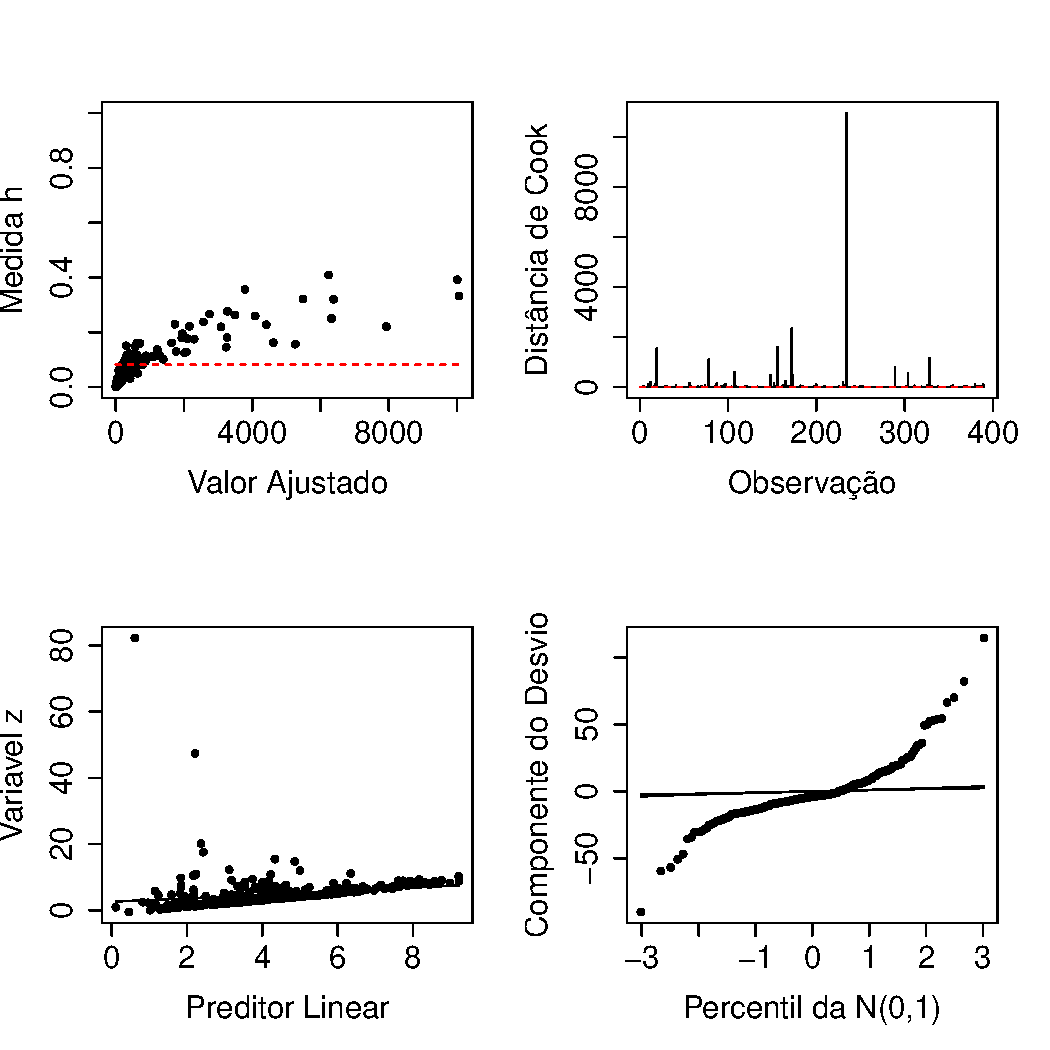
\includegraphics[width=\maxwidth]{figure/unnamed-chunk-8-1} 

\end{knitrout}
\textbf{Figura :} Gráficos de diagnóstico para o modelo sem \_offset\_.

Como é possível observar pelos gráficos da \emph{Figura}, principalmente pelo gráfico de envelope dos resíduos, temos um modelo superdisperso, o que tentaremos resolver acrescentando um \_offset\_.

\subsubsection{\textbf{Modelo com \_Offset\_}}

Para adicionarmos um dado \_offset\_ no modelo vemos que ele pode ser a variável \_pop\_, que indica uma alta variabilidade do tamanho das populações nos municípios. Segue o modelo:

\begin{knitrout}
\definecolor{shadecolor}{rgb}{0.969, 0.969, 0.969}\color{fgcolor}\begin{kframe}
\begin{verbatim}

Call:
glm(formula = dengue ~ CobCondSaud + CobAtencBsca + temp_p90 + 
    precip + umid + ifdm_saude + ifdm_emprend + cobveg + expcosteira + 
    ivc + ExpAnosEstud + urb + maior65 + adultos + dens + offset(log(pop)), 
    family = poisson, data = data)

Deviance Residuals: 
    Min       1Q   Median       3Q      Max  
-76.558   -8.836   -4.680    0.753   71.536  

Coefficients:
               Estimate Std. Error z value Pr(>|z|)    
(Intercept)  -3.457e+01  3.948e-01 -87.546   <2e-16 ***
CobCondSaud  -9.838e-03  2.650e-04 -37.124   <2e-16 ***
CobAtencBsca  5.798e-03  1.979e-04  29.294   <2e-16 ***
temp_p90      4.254e-01  5.316e-03  80.033   <2e-16 ***
precip        9.829e-04  1.445e-05  68.036   <2e-16 ***
umid          1.046e-01  2.729e-03  38.321   <2e-16 ***
ifdm_saude   -3.633e-02  7.469e-04 -48.638   <2e-16 ***
ifdm_emprend -4.018e-02  4.172e-04 -96.307   <2e-16 ***
cobveg       -3.371e-03  2.019e-04 -16.694   <2e-16 ***
expcosteira  -1.374e-02  1.734e-04 -79.256   <2e-16 ***
ivc          -1.743e-02  2.494e-04 -69.905   <2e-16 ***
ExpAnosEstud  1.261e-01  8.573e-03  14.714   <2e-16 ***
urb           1.829e-02  4.362e-04  41.940   <2e-16 ***
maior65       2.850e-02  3.273e-03   8.708   <2e-16 ***
adultos       1.820e-01  4.011e-03  45.363   <2e-16 ***
dens          6.176e-05  6.065e-06  10.183   <2e-16 ***
---
Signif. codes:  0 '***' 0.001 '**' 0.01 '*' 0.05 '.' 0.1 ' ' 1

(Dispersion parameter for poisson family taken to be 1)

    Null deviance: 180512  on 389  degrees of freedom
Residual deviance:  81585  on 374  degrees of freedom
AIC: 83568

Number of Fisher Scoring iterations: 6
\end{verbatim}
\end{kframe}
\end{knitrout}

% FAZER TABELA NO LUGAR DO SGUNK ACIMA DE SER TEMPO
\newpage
Vemos que, ainda que tenhamos adicionado o dado \_offset\_, continuamos com um desvio do resíduo super alto, o que significa que o ajuste segue impróprio para o modelo, o que vamos confirmar com a análise dos gráficos do modelo:

\begin{knitrout}
\definecolor{shadecolor}{rgb}{0.969, 0.969, 0.969}\color{fgcolor}
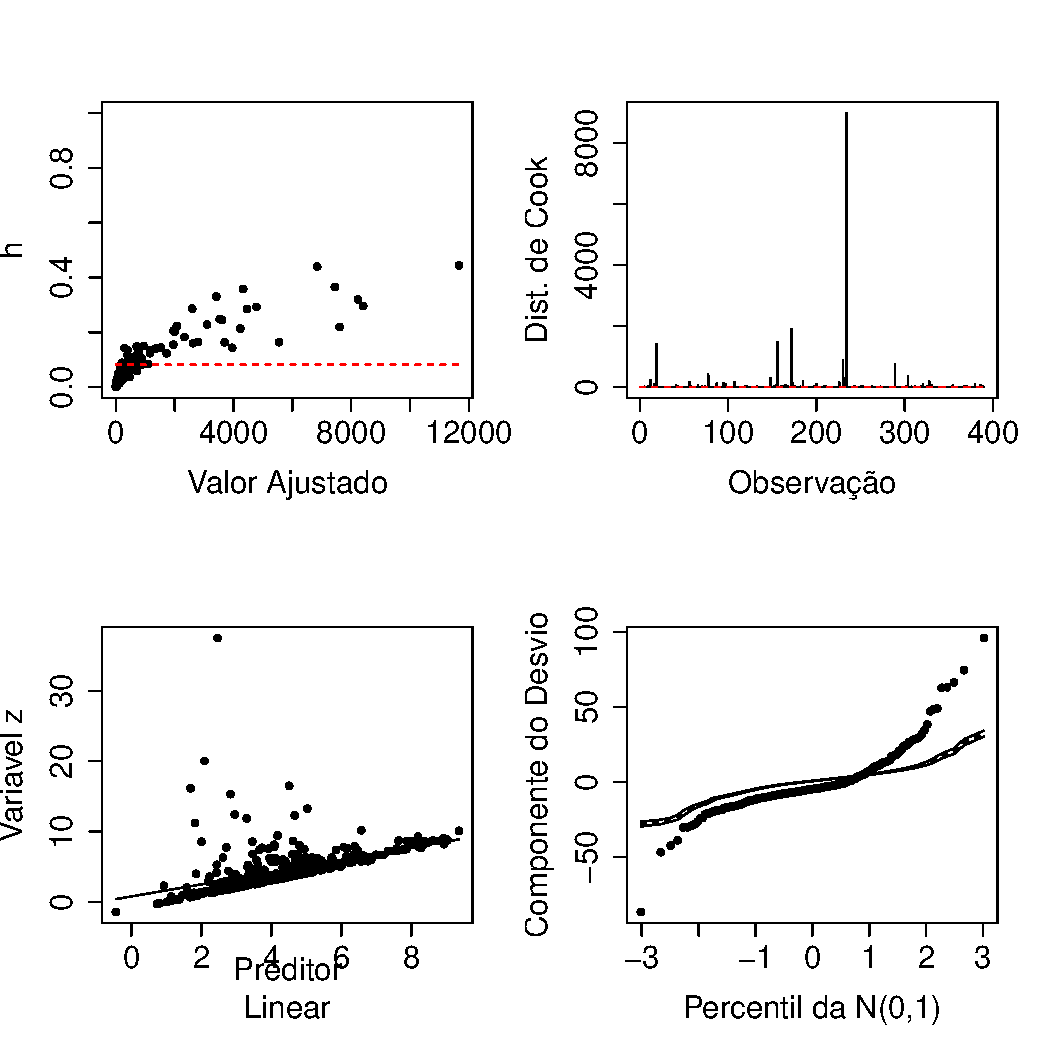
\includegraphics[width=\maxwidth]{figure/unnamed-chunk-10-1} 

\end{knitrout}
\textbf{Figura :} Gráficos de diagnóstico para o modelo com \_offset\_.

\newpage
\subsubsection{\textbf{Interpretação e conclusões}}

Pudemos observar que, mesmo manipulando nosso modelo, continuamos com um ajuste ruim, visto que temos um desvio residual muito maior que os graus de liberdade. Outro indício disso é a sobredispersão observada no gráfico de envelope, o que podemos imaginar que ocorreria, uma vez que temos a média da nossa variável resposta dengue consideravelmente diferente da sua variância, o que não deveria ocorrer, uma vez que a distribuição de Poisson teórica possui média e variância iguais.

Tais constatações nos levam a descartar o modelo Poisson e tentar o ajuste por um modelo Binomial Negativo.

%%%%%%Modelos

\subsection{\textbf{Modelo Binomial Negativo}}
O modelo Binomial Negativo por definição não é MLG, entretanto, possui características muito semelhantes e possui uma boa capacidade de capturar um efeito $E(Y_i)<Var(Y_i)$. Que é exatamente o problema encontrado acima.
\subsubsection{\textbf{Definição do modelo}}
Utilizando uma função de ligação logarítmica temos um modelo inicial utilizando todas as variáveis na forma sistemática abaixo

$$log(\lambda_i)=\alpha+\beta_1{x_1}_i+\beta_2{x_2}_i+\cdots+\beta_{26}{x_{26}}_i$$
\subsubsection{\textbf{Modelo considerando todas covariáveis}}
Ajustando um modelo com todas as 26 covariáveis e realizando a seleção de variáveis pelo método AIC temos suas informações abaixo:
\begin{knitrout}
\definecolor{shadecolor}{rgb}{0.969, 0.969, 0.969}\color{fgcolor}\begin{kframe}
\begin{verbatim}

Call:
glm.nb(formula = dengue ~ CobAtencBsca + temp_p10 + temp + temp_p90 + 
    umid_p10 + umid + alt + ifdm_edu + ifdm_emprend + ivc + urb + 
    menor15 + maior65 + pop + area, data = dados, control = glm.control(maxit = 50), 
    init.theta = 0.6787461656, link = log)

Deviance Residuals: 
    Min       1Q   Median       3Q      Max  
-2.4329  -1.1783  -0.5526   0.1411   2.7976  

Coefficients:
               Estimate Std. Error z value Pr(>|z|)    
(Intercept)   5.133e+00  6.101e+00   0.841 0.400165    
CobAtencBsca -1.062e-02  3.778e-03  -2.811 0.004932 ** 
temp_p10      2.490e+00  3.730e-01   6.677 2.44e-11 ***
temp         -2.995e+00  6.341e-01  -4.723 2.33e-06 ***
temp_p90      5.525e-01  3.284e-01   1.682 0.092510 .  
umid_p10     -5.062e-01  7.104e-02  -7.126 1.03e-12 ***
umid          5.038e-01  9.732e-02   5.176 2.26e-07 ***
alt          -2.248e-03  5.793e-04  -3.881 0.000104 ***
ifdm_edu      4.220e-02  1.823e-02   2.315 0.020639 *  
ifdm_emprend -1.557e-02  7.711e-03  -2.019 0.043449 *  
ivc          -7.831e-03  4.752e-03  -1.648 0.099358 .  
urb           4.974e-02  4.531e-03  10.978  < 2e-16 ***
menor15      -1.197e-01  6.162e-02  -1.943 0.052063 .  
maior65      -1.768e-01  8.322e-02  -2.125 0.033580 *  
pop           6.195e-06  1.003e-06   6.179 6.47e-10 ***
area          5.633e-04  1.368e-04   4.118 3.82e-05 ***
---
Signif. codes:  0 '***' 0.001 '**' 0.01 '*' 0.05 '.' 0.1 ' ' 1

(Dispersion parameter for Negative Binomial(0.6787) family taken to be 1)

    Null deviance: 1482.16  on 389  degrees of freedom
Residual deviance:  457.31  on 374  degrees of freedom
AIC: 3971.4

Number of Fisher Scoring iterations: 1


              Theta:  0.6787 
          Std. Err.:  0.0460 

 2 x log-likelihood:  -3937.3930 
\end{verbatim}
\end{kframe}
\end{knitrout}
Como aconteceu com o Modelo Poisson, é possivel perceber, com base no desvio residual que o ajuste é ruim. Para corrir isso, faremos o mesmo que foi feito com o Modelo Poisson, ou seja, usaremos as 15 variáveis mais correlatadas com a variável resposta, sendo elas:

\begin{itemize}
  \item CobCondSaud
  \item CobAtencBsca
  \item temp\_p$90$
  \item precip
  \item umid
  \item ifdm\_saude
  \item ifdm\_emprend
  \item cobveg
  \item expcosteira
  \item ivc
  \item ExpAnosEstud
  \item urb
  \item maior$65$
  \item adultos
  \item dens
\end{itemize}

\subsubsection{\textbf{Modelo com seleção de covariáveis}}

Com o modelo descrito acima obtivemos, também com a seleção de variáveis pelo \_AIC\_, os seguintes resultados:
\begin{knitrout}
\definecolor{shadecolor}{rgb}{0.969, 0.969, 0.969}\color{fgcolor}\begin{kframe}
\begin{verbatim}

Call:
glm.nb(formula = dengue ~ CobAtencBsca + temp_p90 + ifdm_saude + 
    ifdm_emprend + cobveg + urb + maior65 + pop, data = dados_2013, 
    control = glm.control(maxit = 50), init.theta = 0.9549042419, 
    link = log)

Deviance Residuals: 
    Min       1Q   Median       3Q      Max  
-2.2211  -1.1597  -0.5190   0.5277   1.7196  

Coefficients:
               Estimate Std. Error z value Pr(>|z|)    
(Intercept)  -9.909e+00  2.488e+00  -3.983  6.8e-05 ***
CobAtencBsca -1.731e-02  6.116e-03  -2.830  0.00466 ** 
temp_p90      2.597e-01  1.003e-01   2.590  0.00960 ** 
ifdm_saude    3.859e-02  1.628e-02   2.371  0.01773 *  
ifdm_emprend  1.990e-02  1.385e-02   1.436  0.15091    
cobveg       -1.410e-02  4.493e-03  -3.139  0.00170 ** 
urb           5.752e-02  8.886e-03   6.473  9.6e-11 ***
maior65       2.543e-01  8.215e-02   3.095  0.00197 ** 
pop           4.355e-06  1.837e-06   2.371  0.01776 *  
---
Signif. codes:  0 '***' 0.001 '**' 0.01 '*' 0.05 '.' 0.1 ' ' 1

(Dispersion parameter for Negative Binomial(0.9549) family taken to be 1)

    Null deviance: 387.550  on 77  degrees of freedom
Residual deviance:  89.209  on 69  degrees of freedom
AIC: 912.9

Number of Fisher Scoring iterations: 1


              Theta:  0.955 
          Std. Err.:  0.142 

 2 x log-likelihood:  -892.899 
\end{verbatim}
\end{kframe}
\end{knitrout}
Perceba que, com a escolha de variáveis acima, melhoramos bastante o ajuste do modelo. Gerando os gráficos para o modelo acima, obtemos:
\begin{knitrout}
\definecolor{shadecolor}{rgb}{0.969, 0.969, 0.969}\color{fgcolor}\begin{kframe}
\begin{verbatim}
Negative binomial model (using MASS package) 
\end{verbatim}
\end{kframe}
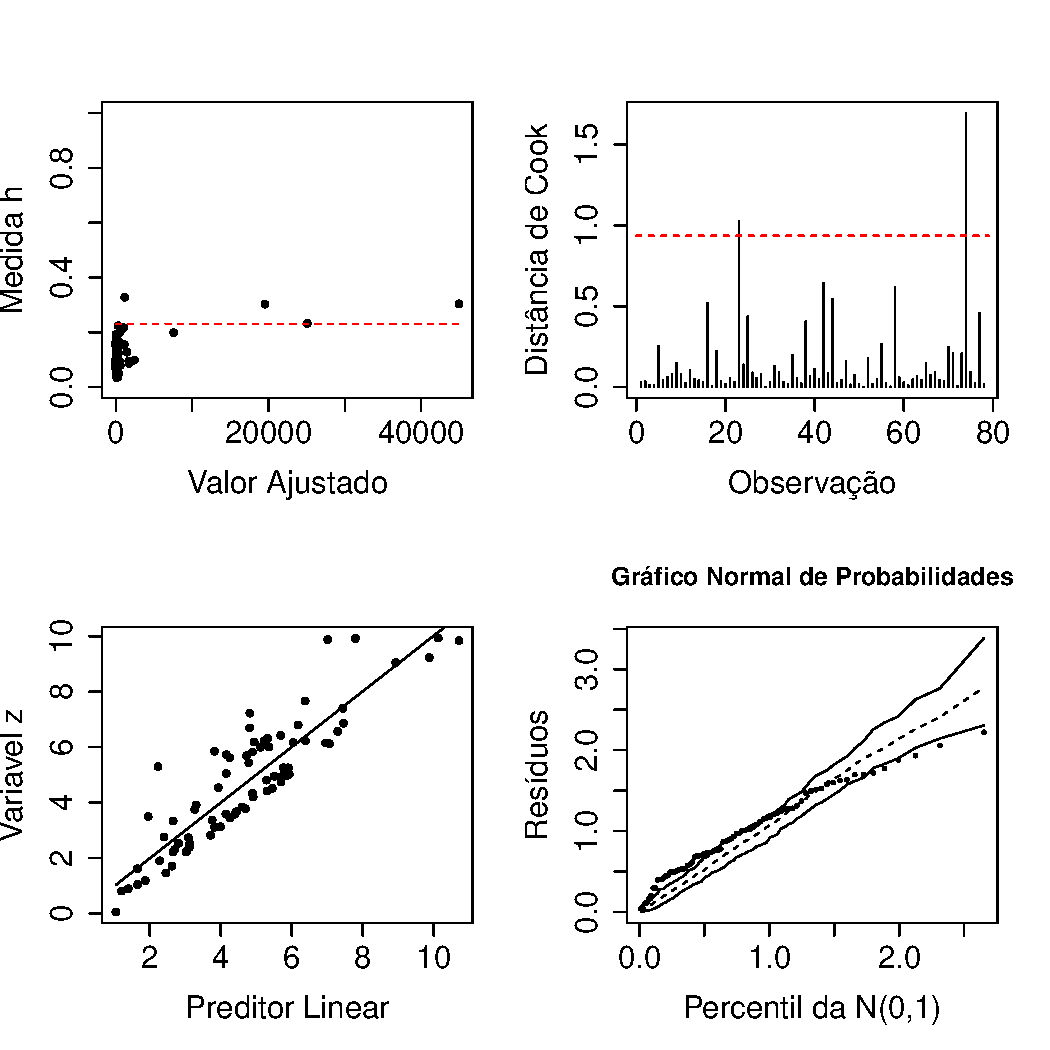
\includegraphics[width=\maxwidth]{figure/unnamed-chunk-14-1} 

\end{knitrout}

\subsubsection{\textbf{Modelo com \_Offset\_}}
Agora, colocando a variável \_pop\_ como \_Offset\_
\begin{knitrout}
\definecolor{shadecolor}{rgb}{0.969, 0.969, 0.969}\color{fgcolor}\begin{kframe}
\begin{verbatim}

Call:
glm.nb(formula = dengue ~ temp_p90 + umid + cobveg + urb + maior65 + 
    adultos + offset(log(pop)), data = dados_2013, control = glm.control(maxit = 50), 
    init.theta = 1.108820464, link = log)

Deviance Residuals: 
    Min       1Q   Median       3Q      Max  
-2.4896  -1.0525  -0.4003   0.4286   1.8971  

Coefficients:
              Estimate Std. Error z value Pr(>|z|)    
(Intercept) -22.743600   6.472959  -3.514 0.000442 ***
temp_p90      0.340296   0.091139   3.734 0.000189 ***
umid         -0.131944   0.085253  -1.548 0.121702    
cobveg       -0.012231   0.004026  -3.038 0.002381 ** 
urb           0.041645   0.006909   6.028 1.66e-09 ***
maior65       0.303516   0.071226   4.261 2.03e-05 ***
adultos       0.205808   0.080866   2.545 0.010926 *  
---
Signif. codes:  0 '***' 0.001 '**' 0.01 '*' 0.05 '.' 0.1 ' ' 1

(Dispersion parameter for Negative Binomial(1.1088) family taken to be 1)

    Null deviance: 185.528  on 77  degrees of freedom
Residual deviance:  87.661  on 71  degrees of freedom
AIC: 895.02

Number of Fisher Scoring iterations: 1


              Theta:  1.109 
          Std. Err.:  0.168 

 2 x log-likelihood:  -879.015 
\end{verbatim}
\end{kframe}
\end{knitrout}
A escolha de deixar a variável \_pop\_ como \_Offset\_ melhorou o ajuste do modelo, visto que o desvio residual se aproximou um pouco mais dos graus de liberdade, abaixo, temos os gráficos do modelo com \_Offset\_:
\begin{knitrout}
\definecolor{shadecolor}{rgb}{0.969, 0.969, 0.969}\color{fgcolor}\begin{kframe}
\begin{verbatim}
Negative binomial model (using MASS package) 
\end{verbatim}
\end{kframe}
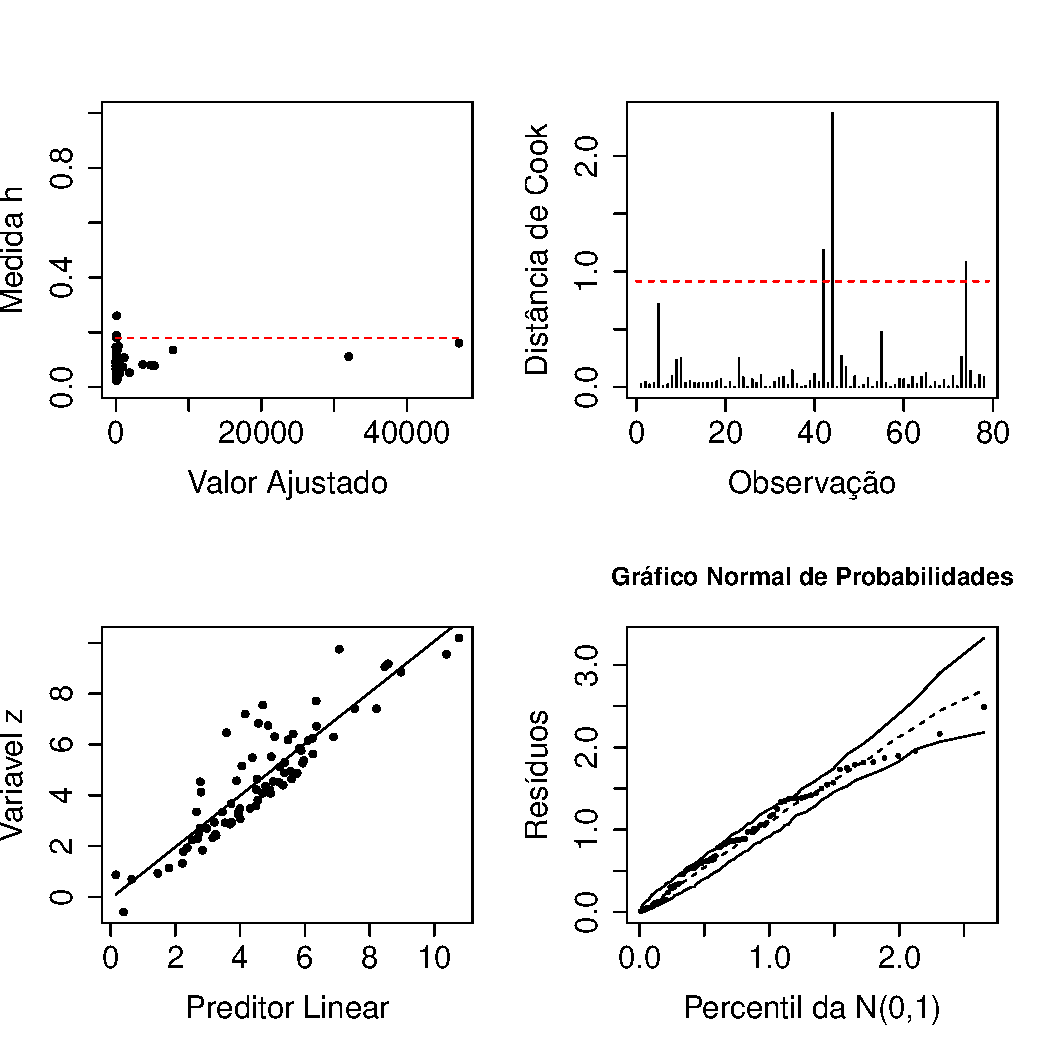
\includegraphics[width=\maxwidth]{figure/unnamed-chunk-16-1} 

\end{knitrout}
\subsubsection{\textbf{Sobre a remoção de pontos influentes}}
Usando a funçao identify, identificamos pontos influentes, entretanto, preferimos por não remove-los no modelo final, já que em nosso subset temos apenas 78 linhas.
Abaixo, alguns resultados que obtivemos na remoção de alguns pontos influentes:




\begin{knitrout}
\definecolor{shadecolor}{rgb}{0.969, 0.969, 0.969}\color{fgcolor}\begin{kframe}
\begin{verbatim}

Call:
glm.nb(formula = dengue ~ CobAtencBsca + temp_p90 + cobveg + 
    urb + maior65 + adultos + offset(log(pop)), data = dados_2013_1, 
    control = glm.control(maxit = 50), init.theta = 1.198029355, 
    link = log)

Deviance Residuals: 
    Min       1Q   Median       3Q      Max  
-2.5633  -1.1437  -0.4232   0.3603   2.2826  

Coefficients:
               Estimate Std. Error z value Pr(>|z|)    
(Intercept)  -34.285911   4.970307  -6.898 5.27e-12 ***
CobAtencBsca  -0.008437   0.005242  -1.609  0.10753    
temp_p90       0.366814   0.087693   4.183 2.88e-05 ***
cobveg        -0.008306   0.003977  -2.089  0.03674 *  
urb            0.035152   0.006475   5.429 5.66e-08 ***
maior65        0.298576   0.068929   4.332 1.48e-05 ***
adultos        0.228635   0.070673   3.235  0.00122 ** 
---
Signif. codes:  0 '***' 0.001 '**' 0.01 '*' 0.05 '.' 0.1 ' ' 1

(Dispersion parameter for Negative Binomial(1.198) family taken to be 1)

    Null deviance: 196.137  on 76  degrees of freedom
Residual deviance:  85.601  on 70  degrees of freedom
AIC: 872.8

Number of Fisher Scoring iterations: 1


              Theta:  1.198 
          Std. Err.:  0.184 

 2 x log-likelihood:  -856.795 
Negative binomial model (using MASS package) 
\end{verbatim}
\end{kframe}
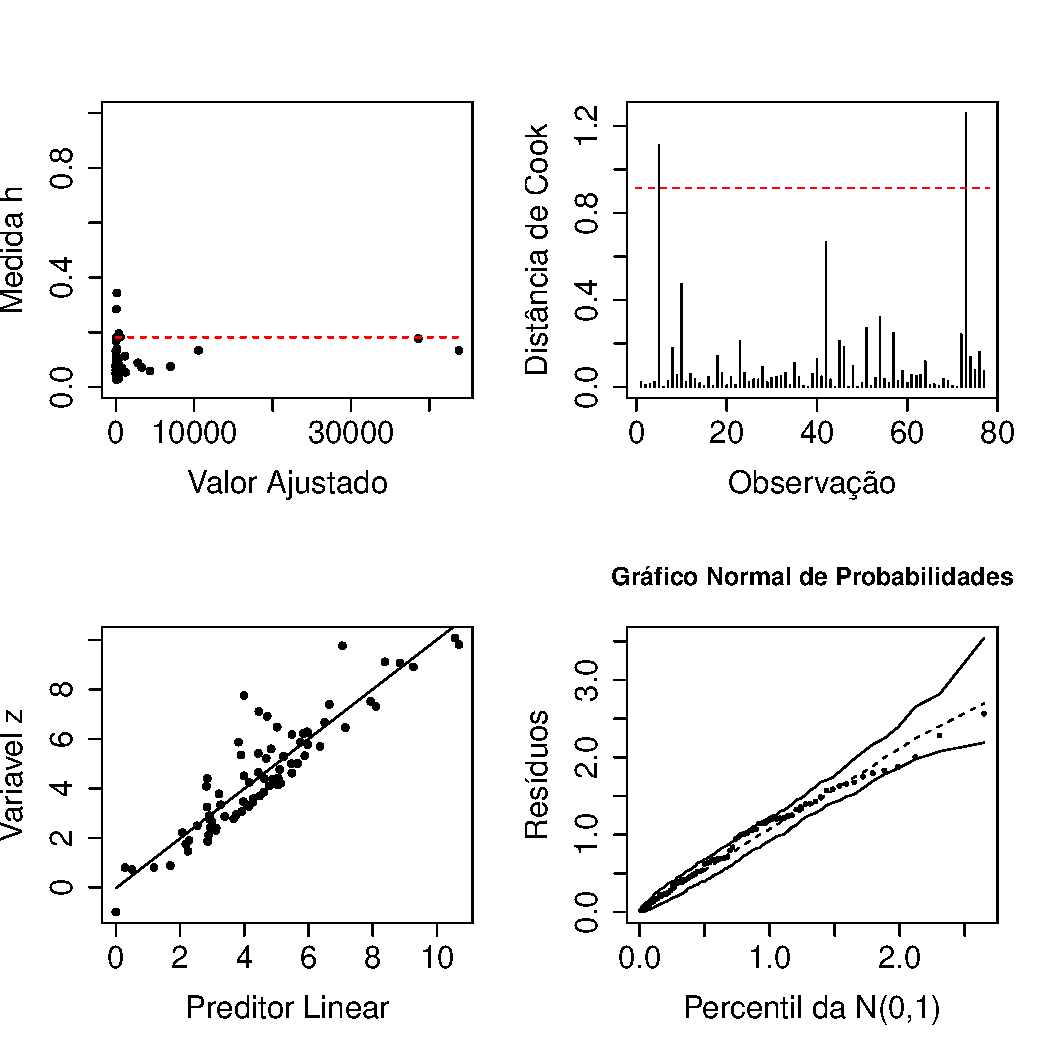
\includegraphics[width=\maxwidth]{figure/unnamed-chunk-19-1} 

\end{knitrout}

\textbf{Figura :} Gráficos de diagnóstico para uma remoção.




\begin{knitrout}
\definecolor{shadecolor}{rgb}{0.969, 0.969, 0.969}\color{fgcolor}\begin{kframe}
\begin{verbatim}

Call:
glm.nb(formula = dengue ~ CobAtencBsca + temp_p90 + cobveg + 
    urb + maior65 + adultos + offset(log(pop)), data = dados_2013_1, 
    control = glm.control(maxit = 50), init.theta = 1.253312012, 
    link = log)

Deviance Residuals: 
    Min       1Q   Median       3Q      Max  
-2.5909  -1.1703  -0.4457   0.3656   2.4699  

Coefficients:
               Estimate Std. Error z value Pr(>|z|)    
(Intercept)  -31.113766   4.886489  -6.367 1.92e-10 ***
CobAtencBsca  -0.009940   0.005143  -1.933  0.05326 .  
temp_p90       0.366527   0.085911   4.266 1.99e-05 ***
cobveg        -0.007076   0.003907  -1.811  0.07013 .  
urb            0.032614   0.006369   5.121 3.05e-07 ***
maior65        0.340456   0.068831   4.946 7.56e-07 ***
adultos        0.179964   0.069549   2.588  0.00967 ** 
---
Signif. codes:  0 '***' 0.001 '**' 0.01 '*' 0.05 '.' 0.1 ' ' 1

(Dispersion parameter for Negative Binomial(1.2533) family taken to be 1)

    Null deviance: 191.231  on 75  degrees of freedom
Residual deviance:  84.312  on 69  degrees of freedom
AIC: 849.46

Number of Fisher Scoring iterations: 1


              Theta:  1.253 
          Std. Err.:  0.196 

 2 x log-likelihood:  -833.462 
Negative binomial model (using MASS package) 
\end{verbatim}
\end{kframe}
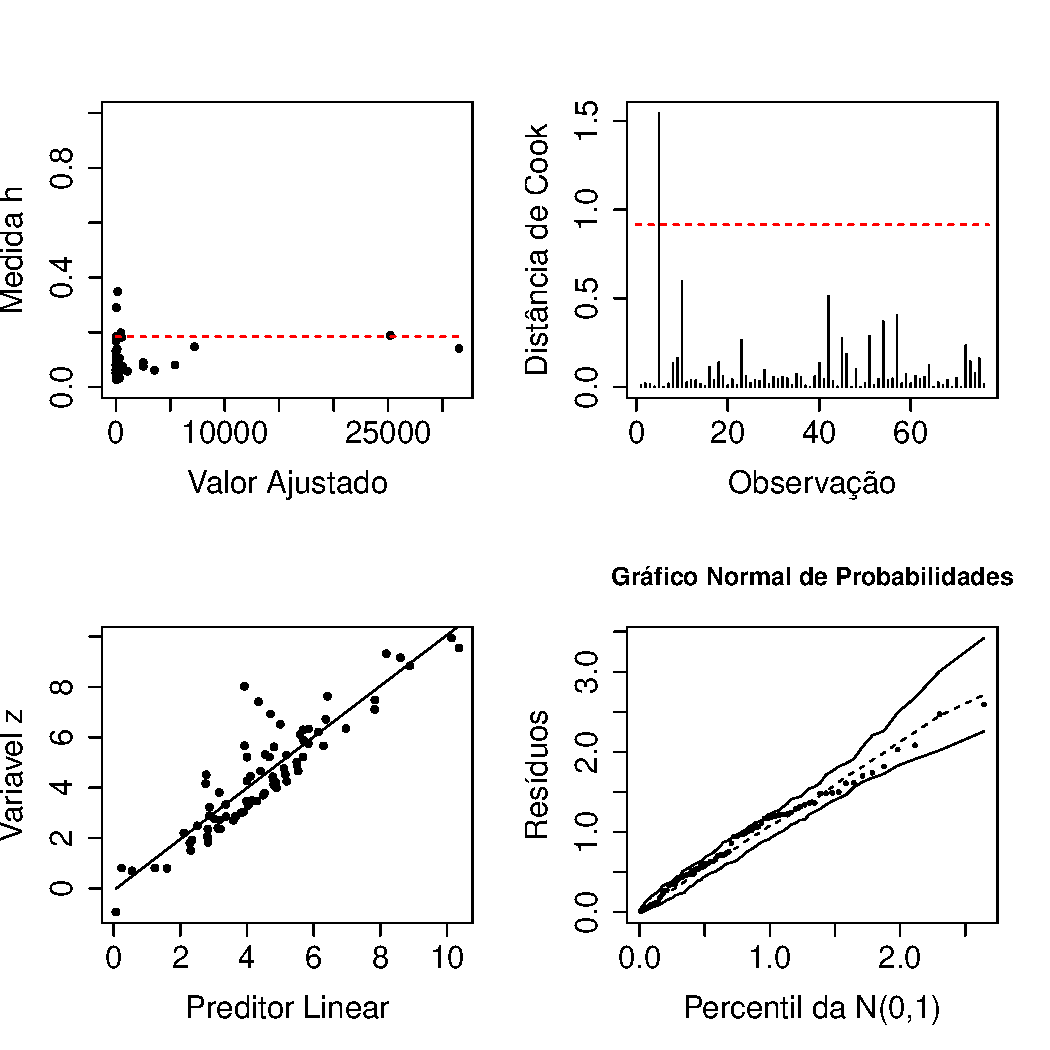
\includegraphics[width=\maxwidth]{figure/unnamed-chunk-22-1} 

\end{knitrout}
\textbf{Figura :} Gráficos de diagnóstico para duas remoção.





\begin{knitrout}
\definecolor{shadecolor}{rgb}{0.969, 0.969, 0.969}\color{fgcolor}\begin{kframe}
\begin{verbatim}

Call:
glm.nb(formula = dengue ~ temp_p90 + ifdm_emprend + urb + maior65 + 
    offset(log(pop)), data = dados_2013_1, control = glm.control(maxit = 50), 
    init.theta = 1.325796543, link = log)

Deviance Residuals: 
    Min       1Q   Median       3Q      Max  
-2.4953  -1.0957  -0.4375   0.4739   2.1774  

Coefficients:
               Estimate Std. Error z value Pr(>|z|)    
(Intercept)  -20.622947   2.066536  -9.979  < 2e-16 ***
temp_p90       0.306737   0.078022   3.931 8.44e-05 ***
ifdm_emprend   0.029342   0.010969   2.675  0.00748 ** 
urb            0.034786   0.006468   5.378 7.53e-08 ***
maior65        0.360962   0.070642   5.110 3.23e-07 ***
---
Signif. codes:  0 '***' 0.001 '**' 0.01 '*' 0.05 '.' 0.1 ' ' 1

(Dispersion parameter for Negative Binomial(1.3258) family taken to be 1)

    Null deviance: 198.864  on 74  degrees of freedom
Residual deviance:  82.865  on 70  degrees of freedom
AIC: 826.49

Number of Fisher Scoring iterations: 1


              Theta:  1.326 
          Std. Err.:  0.210 

 2 x log-likelihood:  -814.486 
Negative binomial model (using MASS package) 
\end{verbatim}
\end{kframe}
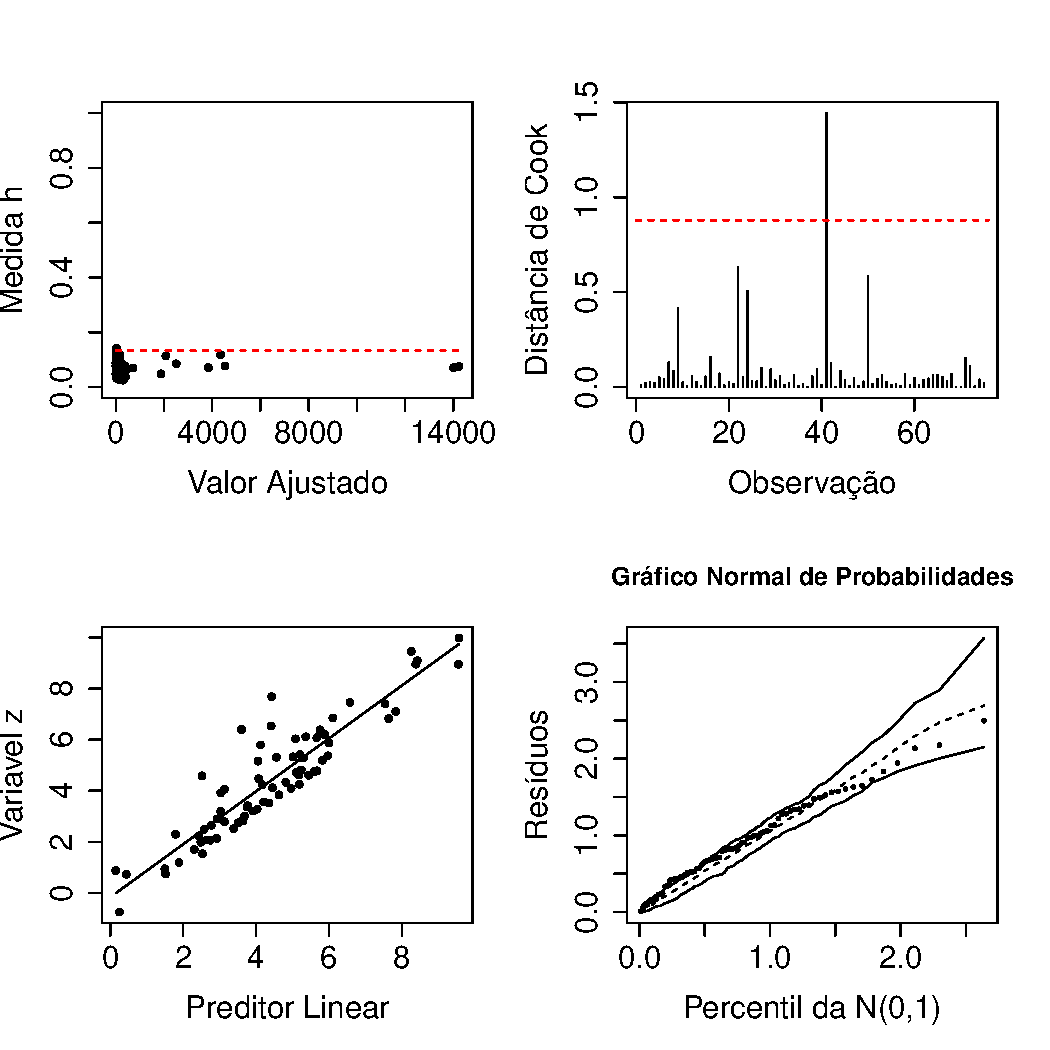
\includegraphics[width=\maxwidth]{figure/unnamed-chunk-25-1} 

\end{knitrout}
\textbf{Figura :} Gráficos de diagnóstico para tres remoções.




\begin{knitrout}
\definecolor{shadecolor}{rgb}{0.969, 0.969, 0.969}\color{fgcolor}\begin{kframe}
\begin{verbatim}

Call:
glm.nb(formula = dengue ~ temp_p90 + ifdm_emprend + urb + maior65 + 
    offset(log(pop)), data = dados_2013_1, control = glm.control(maxit = 50), 
    init.theta = 1.392919725, link = log)

Deviance Residuals: 
    Min       1Q   Median       3Q      Max  
-2.4316  -1.1139  -0.2938   0.4929   2.4241  

Coefficients:
              Estimate Std. Error z value Pr(>|z|)    
(Intercept)  -19.31992    2.03987  -9.471  < 2e-16 ***
temp_p90       0.26653    0.07660   3.479 0.000503 ***
ifdm_emprend   0.02567    0.01081   2.374 0.017616 *  
urb            0.04005    0.00651   6.152 7.65e-10 ***
maior65        0.31144    0.07106   4.383 1.17e-05 ***
---
Signif. codes:  0 '***' 0.001 '**' 0.01 '*' 0.05 '.' 0.1 ' ' 1

(Dispersion parameter for Negative Binomial(1.3929) family taken to be 1)

    Null deviance: 207.600  on 73  degrees of freedom
Residual deviance:  81.419  on 69  degrees of freedom
AIC: 809.81

Number of Fisher Scoring iterations: 1


              Theta:  1.393 
          Std. Err.:  0.224 

 2 x log-likelihood:  -797.807 
Negative binomial model (using MASS package) 
\end{verbatim}
\end{kframe}
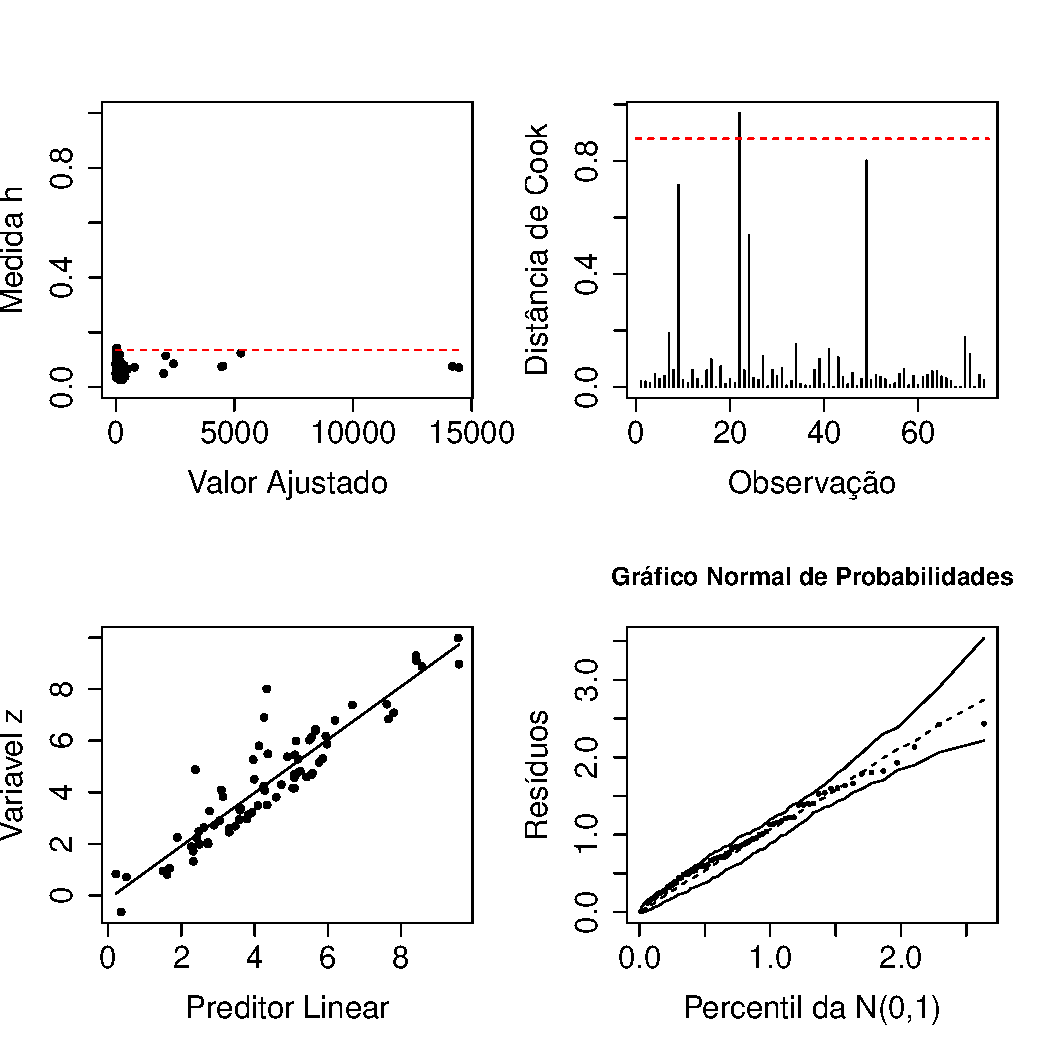
\includegraphics[width=\maxwidth]{figure/unnamed-chunk-28-1} 

\end{knitrout}
\textbf{Figura :} Gráficos de diagnóstico para quatro remoções.


Como optamos por manter os pontos influentes os gráficos de analise ficaram da seguinte forma:


\begin{knitrout}
\definecolor{shadecolor}{rgb}{0.969, 0.969, 0.969}\color{fgcolor}\begin{kframe}
\begin{verbatim}
Negative binomial model (using MASS package) 
\end{verbatim}
\end{kframe}
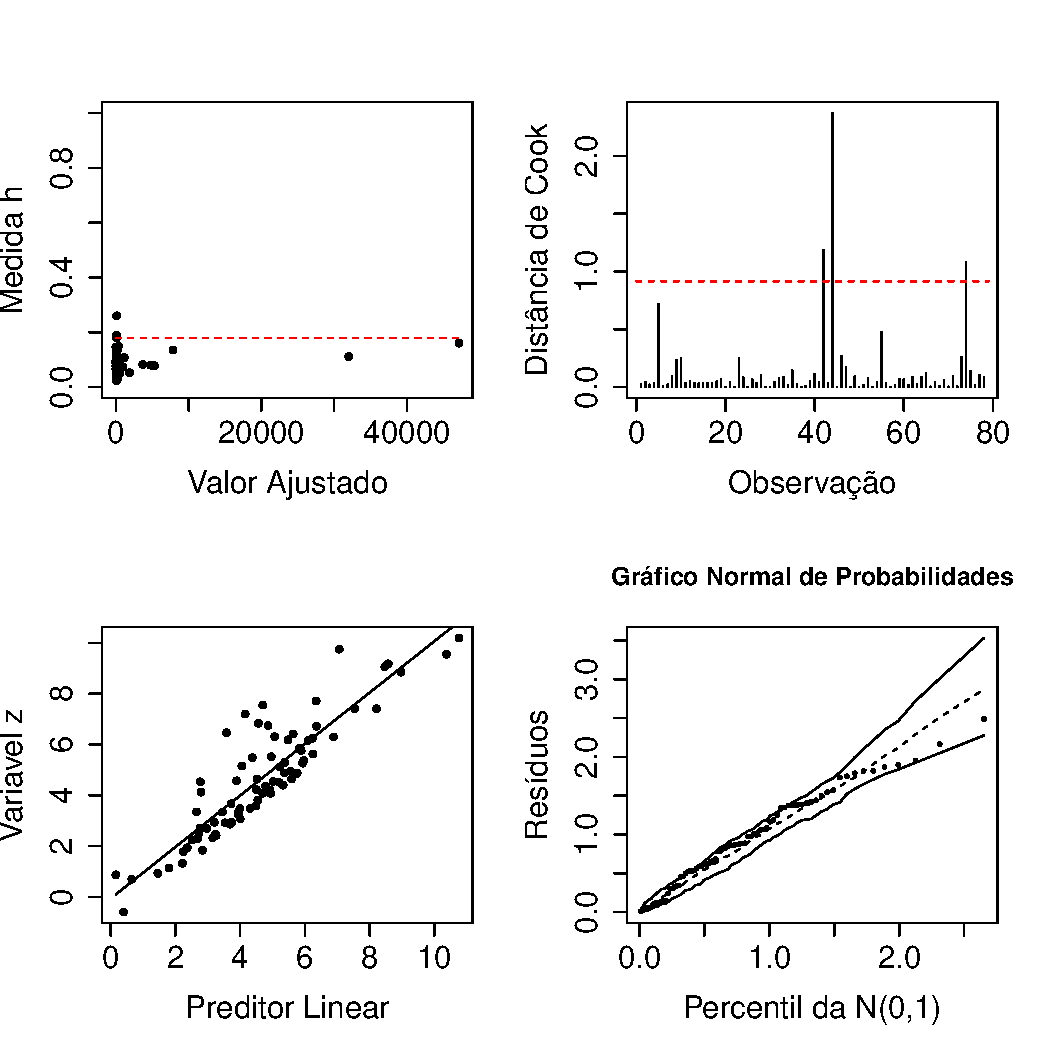
\includegraphics[width=\maxwidth]{figure/unnamed-chunk-30-1} 

\end{knitrout}
Podemos percerber pelos gráficos que o ajuste foi bem feito, muito diferente de quando utilizamos a Poisson.
\subsubsection{\textbf{Interpretação e conclusões}}
Pelo ajuste do modelo final, podemos verificar que de fato, o Modelo Binomial Negativo, se adequou aos dados, já que os dados tinham alta variabilidade em relação média, motivo, que levou o descarte do modelo Poisson.
\end{document}
